\documentclass[]{article}
\usepackage{lmodern}
\usepackage{amssymb,amsmath}
\usepackage{ifxetex,ifluatex}
\usepackage{fixltx2e} % provides \textsubscript
\ifnum 0\ifxetex 1\fi\ifluatex 1\fi=0 % if pdftex
  \usepackage[T1]{fontenc}
  \usepackage[utf8]{inputenc}
\else % if luatex or xelatex
  \ifxetex
    \usepackage{mathspec}
  \else
    \usepackage{fontspec}
  \fi
  \defaultfontfeatures{Ligatures=TeX,Scale=MatchLowercase}
\fi
% use upquote if available, for straight quotes in verbatim environments
\IfFileExists{upquote.sty}{\usepackage{upquote}}{}
% use microtype if available
\IfFileExists{microtype.sty}{%
\usepackage{microtype}
\UseMicrotypeSet[protrusion]{basicmath} % disable protrusion for tt fonts
}{}
\usepackage[margin=1in]{geometry}
\usepackage{hyperref}
\hypersetup{unicode=true,
            pdftitle={Project3},
            pdfauthor={Rongkui Han},
            pdfborder={0 0 0},
            breaklinks=true}
\urlstyle{same}  % don't use monospace font for urls
\usepackage{color}
\usepackage{fancyvrb}
\newcommand{\VerbBar}{|}
\newcommand{\VERB}{\Verb[commandchars=\\\{\}]}
\DefineVerbatimEnvironment{Highlighting}{Verbatim}{commandchars=\\\{\}}
% Add ',fontsize=\small' for more characters per line
\usepackage{framed}
\definecolor{shadecolor}{RGB}{248,248,248}
\newenvironment{Shaded}{\begin{snugshade}}{\end{snugshade}}
\newcommand{\AlertTok}[1]{\textcolor[rgb]{0.94,0.16,0.16}{#1}}
\newcommand{\AnnotationTok}[1]{\textcolor[rgb]{0.56,0.35,0.01}{\textbf{\textit{#1}}}}
\newcommand{\AttributeTok}[1]{\textcolor[rgb]{0.77,0.63,0.00}{#1}}
\newcommand{\BaseNTok}[1]{\textcolor[rgb]{0.00,0.00,0.81}{#1}}
\newcommand{\BuiltInTok}[1]{#1}
\newcommand{\CharTok}[1]{\textcolor[rgb]{0.31,0.60,0.02}{#1}}
\newcommand{\CommentTok}[1]{\textcolor[rgb]{0.56,0.35,0.01}{\textit{#1}}}
\newcommand{\CommentVarTok}[1]{\textcolor[rgb]{0.56,0.35,0.01}{\textbf{\textit{#1}}}}
\newcommand{\ConstantTok}[1]{\textcolor[rgb]{0.00,0.00,0.00}{#1}}
\newcommand{\ControlFlowTok}[1]{\textcolor[rgb]{0.13,0.29,0.53}{\textbf{#1}}}
\newcommand{\DataTypeTok}[1]{\textcolor[rgb]{0.13,0.29,0.53}{#1}}
\newcommand{\DecValTok}[1]{\textcolor[rgb]{0.00,0.00,0.81}{#1}}
\newcommand{\DocumentationTok}[1]{\textcolor[rgb]{0.56,0.35,0.01}{\textbf{\textit{#1}}}}
\newcommand{\ErrorTok}[1]{\textcolor[rgb]{0.64,0.00,0.00}{\textbf{#1}}}
\newcommand{\ExtensionTok}[1]{#1}
\newcommand{\FloatTok}[1]{\textcolor[rgb]{0.00,0.00,0.81}{#1}}
\newcommand{\FunctionTok}[1]{\textcolor[rgb]{0.00,0.00,0.00}{#1}}
\newcommand{\ImportTok}[1]{#1}
\newcommand{\InformationTok}[1]{\textcolor[rgb]{0.56,0.35,0.01}{\textbf{\textit{#1}}}}
\newcommand{\KeywordTok}[1]{\textcolor[rgb]{0.13,0.29,0.53}{\textbf{#1}}}
\newcommand{\NormalTok}[1]{#1}
\newcommand{\OperatorTok}[1]{\textcolor[rgb]{0.81,0.36,0.00}{\textbf{#1}}}
\newcommand{\OtherTok}[1]{\textcolor[rgb]{0.56,0.35,0.01}{#1}}
\newcommand{\PreprocessorTok}[1]{\textcolor[rgb]{0.56,0.35,0.01}{\textit{#1}}}
\newcommand{\RegionMarkerTok}[1]{#1}
\newcommand{\SpecialCharTok}[1]{\textcolor[rgb]{0.00,0.00,0.00}{#1}}
\newcommand{\SpecialStringTok}[1]{\textcolor[rgb]{0.31,0.60,0.02}{#1}}
\newcommand{\StringTok}[1]{\textcolor[rgb]{0.31,0.60,0.02}{#1}}
\newcommand{\VariableTok}[1]{\textcolor[rgb]{0.00,0.00,0.00}{#1}}
\newcommand{\VerbatimStringTok}[1]{\textcolor[rgb]{0.31,0.60,0.02}{#1}}
\newcommand{\WarningTok}[1]{\textcolor[rgb]{0.56,0.35,0.01}{\textbf{\textit{#1}}}}
\usepackage{longtable,booktabs}
\usepackage{graphicx,grffile}
\makeatletter
\def\maxwidth{\ifdim\Gin@nat@width>\linewidth\linewidth\else\Gin@nat@width\fi}
\def\maxheight{\ifdim\Gin@nat@height>\textheight\textheight\else\Gin@nat@height\fi}
\makeatother
% Scale images if necessary, so that they will not overflow the page
% margins by default, and it is still possible to overwrite the defaults
% using explicit options in \includegraphics[width, height, ...]{}
\setkeys{Gin}{width=\maxwidth,height=\maxheight,keepaspectratio}
\IfFileExists{parskip.sty}{%
\usepackage{parskip}
}{% else
\setlength{\parindent}{0pt}
\setlength{\parskip}{6pt plus 2pt minus 1pt}
}
\setlength{\emergencystretch}{3em}  % prevent overfull lines
\providecommand{\tightlist}{%
  \setlength{\itemsep}{0pt}\setlength{\parskip}{0pt}}
\setcounter{secnumdepth}{5}
% Redefines (sub)paragraphs to behave more like sections
\ifx\paragraph\undefined\else
\let\oldparagraph\paragraph
\renewcommand{\paragraph}[1]{\oldparagraph{#1}\mbox{}}
\fi
\ifx\subparagraph\undefined\else
\let\oldsubparagraph\subparagraph
\renewcommand{\subparagraph}[1]{\oldsubparagraph{#1}\mbox{}}
\fi

%%% Use protect on footnotes to avoid problems with footnotes in titles
\let\rmarkdownfootnote\footnote%
\def\footnote{\protect\rmarkdownfootnote}

%%% Change title format to be more compact
\usepackage{titling}

% Create subtitle command for use in maketitle
\providecommand{\subtitle}[1]{
  \posttitle{
    \begin{center}\large#1\end{center}
    }
}

\setlength{\droptitle}{-2em}

  \title{Project3}
    \pretitle{\vspace{\droptitle}\centering\huge}
  \posttitle{\par}
    \author{Rongkui Han}
    \preauthor{\centering\large\emph}
  \postauthor{\par}
      \predate{\centering\large\emph}
  \postdate{\par}
    \date{2/6/2020}


\begin{document}
\maketitle

\hypertarget{propensity-score-matching}{%
\subsection{Propensity Score matching}\label{propensity-score-matching}}

\begin{Shaded}
\begin{Highlighting}[]
\KeywordTok{library}\NormalTok{(MatchIt)}
\end{Highlighting}
\end{Shaded}

\begin{verbatim}
## Warning: package 'MatchIt' was built under R version 3.6.2
\end{verbatim}

\begin{Shaded}
\begin{Highlighting}[]
\KeywordTok{library}\NormalTok{(dplyr)}
\end{Highlighting}
\end{Shaded}

\begin{verbatim}
## 
## Attaching package: 'dplyr'
\end{verbatim}

\begin{verbatim}
## The following objects are masked from 'package:stats':
## 
##     filter, lag
\end{verbatim}

\begin{verbatim}
## The following objects are masked from 'package:base':
## 
##     intersect, setdiff, setequal, union
\end{verbatim}

\begin{Shaded}
\begin{Highlighting}[]
\KeywordTok{library}\NormalTok{(ggplot2)}
\KeywordTok{library}\NormalTok{(lme4)}
\end{Highlighting}
\end{Shaded}

\begin{verbatim}
## Warning: package 'lme4' was built under R version 3.6.2
\end{verbatim}

\begin{verbatim}
## Loading required package: Matrix
\end{verbatim}

\begin{Shaded}
\begin{Highlighting}[]
\KeywordTok{library}\NormalTok{(AER)}
\end{Highlighting}
\end{Shaded}

\begin{verbatim}
## Warning: package 'AER' was built under R version 3.6.2
\end{verbatim}

\begin{verbatim}
## Loading required package: car
\end{verbatim}

\begin{verbatim}
## Loading required package: carData
\end{verbatim}

\begin{verbatim}
## Registered S3 methods overwritten by 'car':
##   method                          from
##   influence.merMod                lme4
##   cooks.distance.influence.merMod lme4
##   dfbeta.influence.merMod         lme4
##   dfbetas.influence.merMod        lme4
\end{verbatim}

\begin{verbatim}
## 
## Attaching package: 'car'
\end{verbatim}

\begin{verbatim}
## The following object is masked from 'package:dplyr':
## 
##     recode
\end{verbatim}

\begin{verbatim}
## Loading required package: lmtest
\end{verbatim}

\begin{verbatim}
## Loading required package: zoo
\end{verbatim}

\begin{verbatim}
## 
## Attaching package: 'zoo'
\end{verbatim}

\begin{verbatim}
## The following objects are masked from 'package:base':
## 
##     as.Date, as.Date.numeric
\end{verbatim}

\begin{verbatim}
## Loading required package: sandwich
\end{verbatim}

\begin{verbatim}
## Warning: package 'sandwich' was built under R version 3.6.2
\end{verbatim}

\begin{verbatim}
## Loading required package: survival
\end{verbatim}

\begin{Shaded}
\begin{Highlighting}[]
\KeywordTok{data}\NormalTok{(}\StringTok{"Fatalities"}\NormalTok{)}
\NormalTok{data =}\StringTok{ }\NormalTok{Fatalities}

\CommentTok{#Impute values for missing CA data}
\NormalTok{data[}\DecValTok{28}\NormalTok{,}\DecValTok{15}\NormalTok{] =}\StringTok{ }\KeywordTok{as.factor}\NormalTok{(}\StringTok{"no"}\NormalTok{)}
\NormalTok{data[}\DecValTok{28}\NormalTok{,}\DecValTok{16}\NormalTok{] =}\StringTok{ }\KeywordTok{as.factor}\NormalTok{(}\StringTok{"no"}\NormalTok{)}


\CommentTok{#head(data)}
\CommentTok{#dim(data)}
\NormalTok{data[}\StringTok{'fr'}\NormalTok{] =}\StringTok{ }\NormalTok{data}\OperatorTok{$}\NormalTok{fatal}\OperatorTok{/}\NormalTok{data}\OperatorTok{$}\NormalTok{pop}\OperatorTok{*}\DecValTok{10000}
\end{Highlighting}
\end{Shaded}

\hypertarget{propensity-score-estimation}{%
\subsubsection{Propensity score estimation}\label{propensity-score-estimation}}

We estimate the propensity score by running a logit model (probit also works) where the outcome variable is a binary variable indicating treatment status. What covariates should you include? For the matching to give you a causal estimate in the end, you need to include any covariate that is related to \textbf{both the treatment assignment and potential outcomes}. I choose just a few covariates below---they are unlikely to capture all covariates that should be included. You'll be asked to come up with a potentially better model on your own later.

\begin{Shaded}
\begin{Highlighting}[]
\NormalTok{data}\OperatorTok{$}\NormalTok{jail =}\StringTok{ }\KeywordTok{ifelse}\NormalTok{(data}\OperatorTok{$}\NormalTok{jail }\OperatorTok{==}\StringTok{ 'yes'}\NormalTok{, }\DecValTok{1}\NormalTok{, }\DecValTok{0}\NormalTok{)}
\NormalTok{m_ps =}\StringTok{ }\KeywordTok{glm}\NormalTok{(jail }\OperatorTok{~}\StringTok{ }\NormalTok{year }\OperatorTok{+}\StringTok{ }\NormalTok{spirits }\OperatorTok{+}\StringTok{ }\NormalTok{unemp }\OperatorTok{+}\StringTok{ }\NormalTok{income }\OperatorTok{+}\StringTok{ }\NormalTok{beertax }\OperatorTok{+}\StringTok{ }\NormalTok{baptist }\OperatorTok{+}\StringTok{ }\NormalTok{mormon }\OperatorTok{+}\StringTok{ }\NormalTok{drinkage }\OperatorTok{+}\StringTok{ }\NormalTok{dry }\OperatorTok{+}\StringTok{ }\NormalTok{youngdrivers }\OperatorTok{+}\StringTok{ }\NormalTok{miles }\OperatorTok{+}\StringTok{ }\NormalTok{breath }\OperatorTok{+}\StringTok{ }\NormalTok{service }\OperatorTok{+}\StringTok{ }\NormalTok{pop }\OperatorTok{+}\StringTok{ }\NormalTok{gsp, }\DataTypeTok{family =} \KeywordTok{binomial}\NormalTok{(), }\DataTypeTok{data =}\NormalTok{ data)}
\KeywordTok{summary}\NormalTok{(m_ps)}
\end{Highlighting}
\end{Shaded}

\begin{verbatim}
## 
## Call:
## glm(formula = jail ~ year + spirits + unemp + income + beertax + 
##     baptist + mormon + drinkage + dry + youngdrivers + miles + 
##     breath + service + pop + gsp, family = binomial(), data = data)
## 
## Deviance Residuals: 
##      Min        1Q    Median        3Q       Max  
## -2.58499  -0.28426  -0.07618   0.03965   2.51035  
## 
## Coefficients:
##                Estimate Std. Error z value Pr(>|z|)    
## (Intercept)   2.029e+01  8.080e+00   2.510 0.012057 *  
## year1983      2.364e-02  9.409e-01   0.025 0.979957    
## year1984      1.236e+00  1.049e+00   1.179 0.238330    
## year1985      2.165e+00  1.006e+00   2.152 0.031360 *  
## year1986      2.551e+00  1.096e+00   2.327 0.019943 *  
## year1987      2.889e+00  1.188e+00   2.432 0.015020 *  
## year1988      3.306e+00  1.354e+00   2.442 0.014611 *  
## spirits      -4.801e-02  3.797e-01  -0.126 0.899388    
## unemp         6.375e-01  1.653e-01   3.857 0.000115 ***
## income       -4.207e-04  2.119e-04  -1.986 0.047078 *  
## beertax      -1.375e+00  8.118e-01  -1.693 0.090389 .  
## baptist      -8.571e-02  3.457e-02  -2.479 0.013162 *  
## mormon       -8.178e-02  2.559e-02  -3.196 0.001395 ** 
## drinkage     -8.934e-01  3.066e-01  -2.913 0.003575 ** 
## dry          -7.730e-02  3.832e-02  -2.017 0.043683 *  
## youngdrivers -8.505e+00  1.047e+01  -0.812 0.416839    
## miles         3.649e-05  2.890e-04   0.126 0.899520    
## breathyes    -4.792e+00  8.877e-01  -5.398 6.74e-08 ***
## serviceyes    6.190e+00  1.023e+00   6.052 1.43e-09 ***
## pop          -2.414e-07  9.159e-08  -2.636 0.008386 ** 
## gsp           1.609e+01  8.468e+00   1.900 0.057392 .  
## ---
## Signif. codes:  0 '***' 0.001 '**' 0.01 '*' 0.05 '.' 0.1 ' ' 1
## 
## (Dispersion parameter for binomial family taken to be 1)
## 
##     Null deviance: 398.31  on 335  degrees of freedom
## Residual deviance: 155.09  on 315  degrees of freedom
## AIC: 197.09
## 
## Number of Fisher Scoring iterations: 7
\end{verbatim}

\begin{Shaded}
\begin{Highlighting}[]
\NormalTok{prs_df =}\StringTok{ }\KeywordTok{data.frame}\NormalTok{(}\DataTypeTok{pr_score =} \KeywordTok{predict}\NormalTok{(m_ps, }\DataTypeTok{type =} \StringTok{"response"}\NormalTok{),}
                    \DataTypeTok{jail =}\NormalTok{ m_ps}\OperatorTok{$}\NormalTok{model}\OperatorTok{$}\NormalTok{jail)}
\CommentTok{#head(prs_df)}
\CommentTok{#dim(prs_df)}
\end{Highlighting}
\end{Shaded}

\hypertarget{examining-the-region-of-common-support}{%
\paragraph{Examining the region of common support}\label{examining-the-region-of-common-support}}

After estimating the propensity score, it is useful to plot histograms of the estimated propensity scores by treatment status:

\begin{Shaded}
\begin{Highlighting}[]
\NormalTok{labs =}\StringTok{ }\KeywordTok{paste}\NormalTok{(}\StringTok{"Actual jail law implemented:"}\NormalTok{, }\KeywordTok{c}\NormalTok{(}\StringTok{"Yes"}\NormalTok{, }\StringTok{"No"}\NormalTok{))}
\NormalTok{prs_df }\OperatorTok
\StringTok{  }\KeywordTok{mutate}\NormalTok{(}\DataTypeTok{jail =} \KeywordTok{ifelse}\NormalTok{(jail }\OperatorTok{==}\StringTok{ }\DecValTok{1}\NormalTok{, labs[}\DecValTok{1}\NormalTok{], labs[}\DecValTok{2}\NormalTok{])) }\OperatorTok
\StringTok{  }\KeywordTok{ggplot}\NormalTok{(}\KeywordTok{aes}\NormalTok{(}\DataTypeTok{x =}\NormalTok{ pr_score)) }\OperatorTok{+}
\StringTok{  }\KeywordTok{geom_histogram}\NormalTok{(}\DataTypeTok{color =} \StringTok{"white"}\NormalTok{, }\DataTypeTok{bins =} \DecValTok{30}\NormalTok{) }\OperatorTok{+}
\StringTok{  }\KeywordTok{facet_wrap}\NormalTok{(}\OperatorTok{~}\NormalTok{jail) }\OperatorTok{+}
\StringTok{  }\KeywordTok{xlab}\NormalTok{(}\StringTok{"Probability of implementing mandatory jail sentence"}\NormalTok{) }\OperatorTok{+}
\StringTok{  }\KeywordTok{theme_bw}\NormalTok{()}
\end{Highlighting}
\end{Shaded}

\includegraphics{Project3_Rongkui_files/figure-latex/unnamed-chunk-5-1.pdf}

\hypertarget{executing-a-matching-algorithm}{%
\subsection{Executing a matching algorithm}\label{executing-a-matching-algorithm}}

A simple method for estimating the treatment effect of Catholic schooling is to restrict the sample to observations within the region of common support, and then to divide the sample within the region of common support into 5 quintiles, based on the estimated propensity score. Within each of these 5 quintiles, we can then estimate the mean difference in student achievement by treatment status. Rubin and others have argued that this is sufficient to eliminate 95\% of the bias due to confounding of treatment status with a covariate.

However, most matching algorithms adopt slightly more complex methods. The method we use below is to find pairs of observations that have very similar propensity scores, but that differ in their treatment status. We use the package MatchIt for this. This package estimates the propensity score in the background and then matches observations based on the method of choice (``nearest'' in this case).

\begin{Shaded}
\begin{Highlighting}[]
\NormalTok{data_cov =}\StringTok{ }\KeywordTok{c}\NormalTok{(}\StringTok{"year"}\NormalTok{, }\StringTok{"spirits"}\NormalTok{ , }\StringTok{"unemp"}\NormalTok{ , }\StringTok{"income"}\NormalTok{ , }\StringTok{"beertax"}\NormalTok{ , }\StringTok{"baptist"}\NormalTok{ , }\StringTok{"mormon"}\NormalTok{ , }\StringTok{"drinkage"}\NormalTok{ , }\StringTok{"dry"}\NormalTok{ , }\StringTok{"youngdrivers"}\NormalTok{ , }\StringTok{"miles"}\NormalTok{ , }\StringTok{"breath"}\NormalTok{ , }\StringTok{"service"}\NormalTok{ , }\StringTok{"pop"}\NormalTok{ , }\StringTok{"gsp"}\NormalTok{)}

\NormalTok{mod_match =}\StringTok{ }\KeywordTok{matchit}\NormalTok{(jail }\OperatorTok{~}\StringTok{ }\NormalTok{year }\OperatorTok{+}\StringTok{ }\NormalTok{spirits }\OperatorTok{+}\StringTok{ }\NormalTok{unemp }\OperatorTok{+}\StringTok{ }\NormalTok{income }\OperatorTok{+}\StringTok{ }\NormalTok{beertax }\OperatorTok{+}\StringTok{ }\NormalTok{baptist }\OperatorTok{+}\StringTok{ }\NormalTok{mormon }\OperatorTok{+}\StringTok{ }\NormalTok{drinkage }\OperatorTok{+}\StringTok{ }\NormalTok{dry }\OperatorTok{+}\StringTok{ }\NormalTok{youngdrivers }\OperatorTok{+}\StringTok{ }\NormalTok{miles }\OperatorTok{+}\StringTok{ }\NormalTok{breath }\OperatorTok{+}\StringTok{ }\NormalTok{service }\OperatorTok{+}\StringTok{ }\NormalTok{pop }\OperatorTok{+}\StringTok{ }\NormalTok{gsp, }\DataTypeTok{method =} \StringTok{"nearest"}\NormalTok{, }\DataTypeTok{data =}\NormalTok{ data)}

\NormalTok{dta_m =}\StringTok{ }\KeywordTok{match.data}\NormalTok{(mod_match)}
\CommentTok{#dim(dta_m)}
\end{Highlighting}
\end{Shaded}

\hypertarget{examining-covariate-balance-in-the-matched-sample}{%
\subsection{Examining covariate balance in the matched sample}\label{examining-covariate-balance-in-the-matched-sample}}

We'll do three things to assess covariate balance in the matched sample:

\begin{itemize}
\tightlist
\item
  visual inspection
\item
  t-tests of difference-in-means
\item
  computation of the average absolute standardized difference (``standardized imbalance'')
\end{itemize}

\begin{Shaded}
\begin{Highlighting}[]
\NormalTok{fn_bal <-}\StringTok{ }\ControlFlowTok{function}\NormalTok{(dta, variable) \{}
\NormalTok{  dta}\OperatorTok{$}\NormalTok{variable <-}\StringTok{ }\NormalTok{dta[, variable]}
\NormalTok{  dta}\OperatorTok{$}\NormalTok{jail <-}\StringTok{ }\KeywordTok{as.factor}\NormalTok{(dta}\OperatorTok{$}\NormalTok{jail)}
\NormalTok{  support <-}\StringTok{ }\KeywordTok{c}\NormalTok{(}\KeywordTok{min}\NormalTok{(dta}\OperatorTok{$}\NormalTok{variable), }\KeywordTok{max}\NormalTok{(dta}\OperatorTok{$}\NormalTok{variable))}
  \KeywordTok{ggplot}\NormalTok{(dta, }\KeywordTok{aes}\NormalTok{(}\DataTypeTok{x =}\NormalTok{ distance, }\DataTypeTok{y =}\NormalTok{ variable, }\DataTypeTok{color =}\NormalTok{ jail)) }\OperatorTok{+}
\StringTok{    }\KeywordTok{geom_point}\NormalTok{(}\DataTypeTok{alpha =} \FloatTok{0.2}\NormalTok{, }\DataTypeTok{size =} \FloatTok{1.3}\NormalTok{) }\OperatorTok{+}
\StringTok{    }\KeywordTok{geom_smooth}\NormalTok{(}\DataTypeTok{method =} \StringTok{"loess"}\NormalTok{, }\DataTypeTok{se =}\NormalTok{ F) }\OperatorTok{+}
\StringTok{    }\KeywordTok{xlab}\NormalTok{(}\StringTok{"Propensity score"}\NormalTok{) }\OperatorTok{+}
\StringTok{    }\KeywordTok{ylab}\NormalTok{(variable) }\OperatorTok{+}
\StringTok{    }\KeywordTok{theme_bw}\NormalTok{() }\OperatorTok{+}
\StringTok{    }\KeywordTok{ylim}\NormalTok{(support)}
\NormalTok{\}}

\KeywordTok{library}\NormalTok{(gridExtra)}
\end{Highlighting}
\end{Shaded}

\begin{verbatim}
## 
## Attaching package: 'gridExtra'
\end{verbatim}

\begin{verbatim}
## The following object is masked from 'package:dplyr':
## 
##     combine
\end{verbatim}

\begin{Shaded}
\begin{Highlighting}[]
\KeywordTok{grid.arrange}\NormalTok{(}
   \CommentTok{#fn_bal(dta_m, "year"),}
   \KeywordTok{fn_bal}\NormalTok{(dta_m, }\StringTok{"spirits"}\NormalTok{),}
   \KeywordTok{fn_bal}\NormalTok{(dta_m, }\StringTok{"unemp"}\NormalTok{),}
   \KeywordTok{fn_bal}\NormalTok{(dta_m, }\StringTok{"income"}\NormalTok{), }\CommentTok{#+ theme(legend.position = "none"),}
   \KeywordTok{fn_bal}\NormalTok{(dta_m, }\StringTok{"beertax"}\NormalTok{),}
   \CommentTok{#fn_bal(dta_m, "baptist"),}
   \CommentTok{#fn_bal(dta_m, "mormon"),}
   \KeywordTok{fn_bal}\NormalTok{(dta_m, }\StringTok{"drinkage"}\NormalTok{),}
   \KeywordTok{fn_bal}\NormalTok{(dta_m, }\StringTok{"dry"}\NormalTok{),}
   \KeywordTok{fn_bal}\NormalTok{(dta_m, }\StringTok{"youngdrivers"}\NormalTok{),}
   \KeywordTok{fn_bal}\NormalTok{(dta_m, }\StringTok{"miles"}\NormalTok{),}
   \CommentTok{#fn_bal(dta_m, "breath"),}
   \CommentTok{#fn_bal(dta_m, "service"),}
   \KeywordTok{fn_bal}\NormalTok{(dta_m, }\StringTok{"pop"}\NormalTok{),}
   \KeywordTok{fn_bal}\NormalTok{(dta_m, }\StringTok{"gsp"}\NormalTok{),}
   \DataTypeTok{nrow =} \DecValTok{4}\CommentTok{#, widths = c(1, 0.8)}
\NormalTok{)}
\end{Highlighting}
\end{Shaded}

\begin{verbatim}
## Warning: Removed 15 rows containing missing values (geom_smooth).
\end{verbatim}

\includegraphics{Project3_Rongkui_files/figure-latex/unnamed-chunk-7-1.pdf}

\hypertarget{difference-in-means}{%
\paragraph{Difference-in-means}\label{difference-in-means}}

The means below indicate that we have attained a high degree of balance on the five covariates included in the model.

\begin{Shaded}
\begin{Highlighting}[]
\NormalTok{dta_m_mean =}\StringTok{ }\NormalTok{dta_m }\OperatorTok
\StringTok{  }\KeywordTok{group_by}\NormalTok{(jail) }\OperatorTok
\StringTok{  }\KeywordTok{summarise_all}\NormalTok{(}\KeywordTok{funs}\NormalTok{(mean))}
\end{Highlighting}
\end{Shaded}

\begin{verbatim}
## Warning: funs() is soft deprecated as of dplyr 0.8.0
## Please use a list of either functions or lambdas: 
## 
##   # Simple named list: 
##   list(mean = mean, median = median)
## 
##   # Auto named with `tibble::lst()`: 
##   tibble::lst(mean, median)
## 
##   # Using lambdas
##   list(~ mean(., trim = .2), ~ median(., na.rm = TRUE))
## This warning is displayed once per session.
\end{verbatim}

\begin{verbatim}
## Warning in mean.default(state): argument is not numeric or logical: returning NA

## Warning in mean.default(state): argument is not numeric or logical: returning NA
\end{verbatim}

\begin{verbatim}
## Warning in mean.default(year): argument is not numeric or logical: returning NA

## Warning in mean.default(year): argument is not numeric or logical: returning NA
\end{verbatim}

\begin{verbatim}
## Warning in mean.default(breath): argument is not numeric or logical: returning
## NA

## Warning in mean.default(breath): argument is not numeric or logical: returning
## NA
\end{verbatim}

\begin{verbatim}
## Warning in mean.default(service): argument is not numeric or logical: returning
## NA

## Warning in mean.default(service): argument is not numeric or logical: returning
## NA
\end{verbatim}

\begin{Shaded}
\begin{Highlighting}[]
\NormalTok{dta_m_mean =}\StringTok{ }\NormalTok{dta_m_mean[,}\KeywordTok{c}\NormalTok{(}\StringTok{'jail'}\NormalTok{, data_cov)]}
\NormalTok{dta_m_mean}
\end{Highlighting}
\end{Shaded}

\begin{verbatim}
## # A tibble: 2 x 16
##    jail  year spirits unemp income beertax baptist mormon drinkage   dry
##   <dbl> <dbl>   <dbl> <dbl>  <dbl>   <dbl>   <dbl>  <dbl>    <dbl> <dbl>
## 1     0    NA    1.74  7.73 13925.   0.468    7.68   2.53     20.3  5.25
## 2     1    NA    1.70  7.94 13327.   0.485    5.90   6.18     20.3  1.11
## # ... with 6 more variables: youngdrivers <dbl>, miles <dbl>, breath <dbl>,
## #   service <dbl>, pop <dbl>, gsp <dbl>
\end{verbatim}

You can test this more formally using t-tests. Ideally, we should not be able to reject the null hypothesis of no mean difference for each covariate:

Not working:

\begin{Shaded}
\begin{Highlighting}[]
\KeywordTok{lapply}\NormalTok{(data_cov, }\ControlFlowTok{function}\NormalTok{(v) \{}
    \KeywordTok{t.test}\NormalTok{(dta_m[,v] }\OperatorTok{~}\StringTok{ }\NormalTok{dta_m}\OperatorTok{$}\NormalTok{jail)}
\NormalTok{\})}
\end{Highlighting}
\end{Shaded}

\hypertarget{estimating-treatment-effects}{%
\subsection{Estimating treatment effects}\label{estimating-treatment-effects}}

Estimating the treatment effect is simple once we have a matched sample that we are happy with. We can use a t-test:

\begin{Shaded}
\begin{Highlighting}[]
\KeywordTok{with}\NormalTok{(dta_m, }\KeywordTok{t.test}\NormalTok{(fr }\OperatorTok{~}\StringTok{ }\NormalTok{jail))}
\end{Highlighting}
\end{Shaded}

\begin{verbatim}
## 
##  Welch Two Sample t-test
## 
## data:  fr by jail
## t = -2.6653, df = 181.22, p-value = 0.008387
## alternative hypothesis: true difference in means is not equal to 0
## 95 percent confidence interval:
##  -0.40546924 -0.06050356
## sample estimates:
## mean in group 0 mean in group 1 
##        2.061610        2.294596
\end{verbatim}

\begin{Shaded}
\begin{Highlighting}[]
\KeywordTok{summary}\NormalTok{(data}\OperatorTok{$}\NormalTok{fr)}
\end{Highlighting}
\end{Shaded}

\begin{verbatim}
##    Min. 1st Qu.  Median    Mean 3rd Qu.    Max. 
##  0.8212  1.6237  1.9560  2.0404  2.4179  4.2178
\end{verbatim}

Or OLS:

\begin{Shaded}
\begin{Highlighting}[]
\NormalTok{lm_treat1 <-}\StringTok{ }\KeywordTok{lm}\NormalTok{(fr }\OperatorTok{~}\StringTok{ }\NormalTok{jail, }\DataTypeTok{data =}\NormalTok{ dta_m)}
\KeywordTok{summary}\NormalTok{(lm_treat1)}
\end{Highlighting}
\end{Shaded}

\begin{verbatim}
## 
## Call:
## lm(formula = fr ~ jail, data = dta_m)
## 
## Residuals:
##      Min       1Q   Median       3Q      Max 
## -0.93258 -0.43958 -0.06478  0.41301  2.15623 
## 
## Coefficients:
##             Estimate Std. Error t value Pr(>|t|)    
## (Intercept)  2.06161    0.06181  33.353  < 2e-16 ***
## jail         0.23299    0.08742   2.665  0.00837 ** 
## ---
## Signif. codes:  0 '***' 0.001 '**' 0.01 '*' 0.05 '.' 0.1 ' ' 1
## 
## Residual standard error: 0.5993 on 186 degrees of freedom
## Multiple R-squared:  0.03679,    Adjusted R-squared:  0.03161 
## F-statistic: 7.104 on 1 and 186 DF,  p-value: 0.008369
\end{verbatim}

\begin{Shaded}
\begin{Highlighting}[]
\KeywordTok{confint}\NormalTok{(lm_treat1)}
\end{Highlighting}
\end{Shaded}

\begin{verbatim}
##                  2.5 %    97.5 %
## (Intercept) 1.93966687 2.1835523
## jail        0.06053337 0.4054394
\end{verbatim}

\begin{Shaded}
\begin{Highlighting}[]
\NormalTok{lm_orig =}\StringTok{ }\KeywordTok{lm}\NormalTok{(fr }\OperatorTok{~}\StringTok{ }\NormalTok{jail, }\DataTypeTok{data =}\NormalTok{ data)}
\KeywordTok{summary}\NormalTok{(lm_orig)}
\end{Highlighting}
\end{Shaded}

\begin{verbatim}
## 
## Call:
## lm(formula = fr ~ jail, data = data)
## 
## Residuals:
##      Min       1Q   Median       3Q      Max 
## -1.12051 -0.41380 -0.07913  0.33630  2.27612 
## 
## Coefficients:
##             Estimate Std. Error t value Pr(>|t|)    
## (Intercept)  1.94172    0.03526  55.070  < 2e-16 ***
## jail         0.35287    0.06666   5.293 2.18e-07 ***
## ---
## Signif. codes:  0 '***' 0.001 '**' 0.01 '*' 0.05 '.' 0.1 ' ' 1
## 
## Residual standard error: 0.5485 on 334 degrees of freedom
## Multiple R-squared:  0.0774, Adjusted R-squared:  0.07464 
## F-statistic: 28.02 on 1 and 334 DF,  p-value: 2.179e-07
\end{verbatim}

\begin{Shaded}
\begin{Highlighting}[]
\KeywordTok{confint}\NormalTok{(lm_orig)}
\end{Highlighting}
\end{Shaded}

\begin{verbatim}
##                 2.5 %   97.5 %
## (Intercept) 1.8723658 2.011081
## jail        0.2217429 0.484002
\end{verbatim}

\begin{Shaded}
\begin{Highlighting}[]
\KeywordTok{sum}\NormalTok{(dta_m}\OperatorTok{$}\NormalTok{jail }\OperatorTok{==}\StringTok{ }\DecValTok{1}\NormalTok{) }\CommentTok{#94}
\end{Highlighting}
\end{Shaded}

\begin{verbatim}
## [1] 94
\end{verbatim}

\begin{Shaded}
\begin{Highlighting}[]
\KeywordTok{sum}\NormalTok{(dta_m}\OperatorTok{$}\NormalTok{jail }\OperatorTok{==}\StringTok{ }\DecValTok{0}\NormalTok{) }\CommentTok{#94}
\end{Highlighting}
\end{Shaded}

\begin{verbatim}
## [1] 94
\end{verbatim}

\begin{Shaded}
\begin{Highlighting}[]
\KeywordTok{sum}\NormalTok{(data}\OperatorTok{$}\NormalTok{jail }\OperatorTok{==}\StringTok{ }\DecValTok{1}\NormalTok{)}
\end{Highlighting}
\end{Shaded}

\begin{verbatim}
## [1] 94
\end{verbatim}

\begin{Shaded}
\begin{Highlighting}[]
\KeywordTok{sum}\NormalTok{(data}\OperatorTok{$}\NormalTok{jail }\OperatorTok{==}\StringTok{ }\DecValTok{0}\NormalTok{)}
\end{Highlighting}
\end{Shaded}

\begin{verbatim}
## [1] 242
\end{verbatim}

\begin{Shaded}
\begin{Highlighting}[]
\KeywordTok{mean}\NormalTok{(dta_m}\OperatorTok{$}\NormalTok{fr[dta_m}\OperatorTok{$}\NormalTok{jail }\OperatorTok{==}\StringTok{ }\DecValTok{1}\NormalTok{]) }\OperatorTok{-}\StringTok{ }\KeywordTok{mean}\NormalTok{(dta_m}\OperatorTok{$}\NormalTok{fr[dta_m}\OperatorTok{$}\NormalTok{jail }\OperatorTok{==}\StringTok{ }\DecValTok{0}\NormalTok{])}
\end{Highlighting}
\end{Shaded}

\begin{verbatim}
## [1] 0.2329864
\end{verbatim}

\begin{Shaded}
\begin{Highlighting}[]
\KeywordTok{mean}\NormalTok{(dta_m}\OperatorTok{$}\NormalTok{fr[dta_m}\OperatorTok{$}\NormalTok{jail }\OperatorTok{==}\StringTok{ }\DecValTok{0}\NormalTok{])}
\end{Highlighting}
\end{Shaded}

\begin{verbatim}
## [1] 2.06161
\end{verbatim}

\begin{Shaded}
\begin{Highlighting}[]
\KeywordTok{mean}\NormalTok{(dta_m}\OperatorTok{$}\NormalTok{fr[dta_m}\OperatorTok{$}\NormalTok{jail }\OperatorTok{==}\StringTok{ }\DecValTok{1}\NormalTok{])}
\end{Highlighting}
\end{Shaded}

\begin{verbatim}
## [1] 2.294596
\end{verbatim}

\begin{Shaded}
\begin{Highlighting}[]
\KeywordTok{mean}\NormalTok{(data}\OperatorTok{$}\NormalTok{fr[data}\OperatorTok{$}\NormalTok{jail }\OperatorTok{==}\StringTok{ }\DecValTok{1}\NormalTok{]) }\OperatorTok{-}\StringTok{ }\KeywordTok{mean}\NormalTok{(data}\OperatorTok{$}\NormalTok{fr[data}\OperatorTok{$}\NormalTok{jail }\OperatorTok{==}\StringTok{ }\DecValTok{0}\NormalTok{])}
\end{Highlighting}
\end{Shaded}

\begin{verbatim}
## [1] 0.3528725
\end{verbatim}

\begin{Shaded}
\begin{Highlighting}[]
\KeywordTok{plot}\NormalTok{(dta_m}\OperatorTok{$}\NormalTok{year)}
\end{Highlighting}
\end{Shaded}

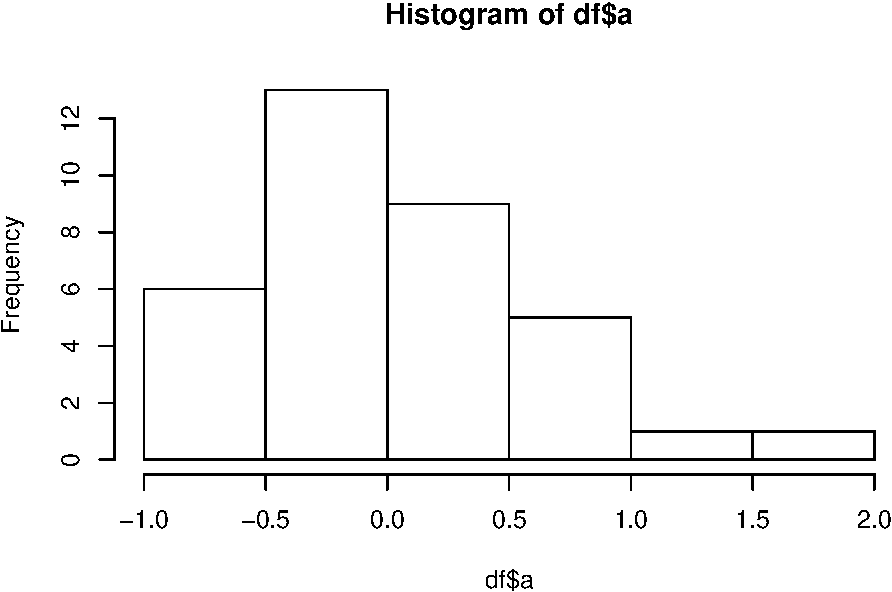
\includegraphics{Project3_Rongkui_files/figure-latex/unnamed-chunk-13-1.pdf}

\begin{Shaded}
\begin{Highlighting}[]
\KeywordTok{plot}\NormalTok{(data}\OperatorTok{$}\NormalTok{year)}
\end{Highlighting}
\end{Shaded}

\includegraphics{Project3_Rongkui_files/figure-latex/unnamed-chunk-13-2.pdf}

\begin{Shaded}
\begin{Highlighting}[]
\CommentTok{#What about if we inlcude state in the linear regression model}

\CommentTok{#Fixed}
\NormalTok{fit1 =}\StringTok{ }\KeywordTok{lm}\NormalTok{(fr }\OperatorTok{~}\StringTok{ }\NormalTok{jail }\OperatorTok{+}\StringTok{ }\NormalTok{state, }\DataTypeTok{data =}\NormalTok{ dta_m)}
\KeywordTok{summary}\NormalTok{(fit1)}
\end{Highlighting}
\end{Shaded}

\begin{verbatim}
## 
## Call:
## lm(formula = fr ~ jail + state, data = dta_m)
## 
## Residuals:
##      Min       1Q   Median       3Q      Max 
## -0.58488 -0.08000 -0.00012  0.08397  0.72365 
## 
## Coefficients:
##             Estimate Std. Error t value Pr(>|t|)    
## (Intercept)  2.33518    0.08524  27.395  < 2e-16 ***
## jail        -0.06008    0.07974  -0.753 0.452344    
## stateaz      0.43080    0.13716   3.141 0.002021 ** 
## statear      0.10871    0.11542   0.942 0.347746    
## stateco     -0.46820    0.11161  -4.195 4.59e-05 ***
## statect     -0.83734    0.12055  -6.946 9.92e-11 ***
## statefl      0.14262    0.11161   1.278 0.203214    
## stateid      0.23649    0.11161   2.119 0.035699 *  
## stateil     -0.98962    0.12786  -7.740 1.23e-12 ***
## statein     -0.48902    0.12055  -4.057 7.89e-05 ***
## stateia     -0.75467    0.13920  -5.422 2.24e-07 ***
## stateks     -0.30544    0.13716  -2.227 0.027411 *  
## stateky     -0.24040    0.20880  -1.151 0.251375    
## statela     -0.15427    0.13716  -1.125 0.262448    
## stateme     -0.40497    0.13716  -2.952 0.003647 ** 
## statema     -1.14107    0.11542  -9.886  < 2e-16 ***
## statemo     -0.35773    0.11161  -3.205 0.001641 ** 
## statemt      0.62792    0.13716   4.578 9.62e-06 ***
## statenv      0.46158    0.13087   3.527 0.000554 ***
## statenh     -0.51029    0.20880  -2.444 0.015657 *  
## statenj     -1.02295    0.11542  -8.863 1.80e-15 ***
## statenm      1.31802    0.11161  11.809  < 2e-16 ***
## stateoh     -0.75038    0.12055  -6.225 4.37e-09 ***
## stateok     -0.29809    0.12786  -2.331 0.021031 *  
## stateor     -0.11512    0.12530  -0.919 0.359658    
## statesc      0.63970    0.14028   4.560 1.04e-05 ***
## statetn      0.12796    0.13716   0.933 0.352322    
## statetx     -0.19784    0.20880  -0.948 0.344863    
## stateut     -0.44887    0.14028  -3.200 0.001670 ** 
## statevt     -0.30874    0.12786  -2.415 0.016922 *  
## statewa     -0.59789    0.13716  -4.359 2.38e-05 ***
## statewv      0.02552    0.13716   0.186 0.852638    
## statewi     -0.72668    0.12786  -5.683 6.43e-08 ***
## statewy      0.94243    0.13716   6.871 1.49e-10 ***
## ---
## Signif. codes:  0 '***' 0.001 '**' 0.01 '*' 0.05 '.' 0.1 ' ' 1
## 
## Residual standard error: 0.1906 on 154 degrees of freedom
## Multiple R-squared:  0.9193, Adjusted R-squared:  0.902 
## F-statistic: 53.18 on 33 and 154 DF,  p-value: < 2.2e-16
\end{verbatim}

\begin{Shaded}
\begin{Highlighting}[]
\CommentTok{#Random}
\NormalTok{fit2 <-}\StringTok{ }\KeywordTok{lmer}\NormalTok{(fr }\OperatorTok{~}\StringTok{ }\NormalTok{jail }\OperatorTok{+}\StringTok{ }\NormalTok{(}\DecValTok{1} \OperatorTok{|}\StringTok{ }\NormalTok{state), }\DataTypeTok{data =}\NormalTok{ dta_m)}
\KeywordTok{summary}\NormalTok{(fit2)}
\end{Highlighting}
\end{Shaded}

\begin{verbatim}
## Linear mixed model fit by REML ['lmerMod']
## Formula: fr ~ jail + (1 | state)
##    Data: dta_m
## 
## REML criterion at convergence: 40.7
## 
## Scaled residuals: 
##     Min      1Q  Median      3Q     Max 
## -2.9762 -0.4294 -0.0078  0.4197  3.8892 
## 
## Random effects:
##  Groups   Name        Variance Std.Dev.
##  state    (Intercept) 0.31749  0.5635  
##  Residual             0.03633  0.1906  
## Number of obs: 188, groups:  state, 33
## 
## Fixed effects:
##             Estimate Std. Error t value
## (Intercept)  2.13359    0.10425  20.465
## jail        -0.01212    0.07466  -0.162
## 
## Correlation of Fixed Effects:
##      (Intr)
## jail -0.301
\end{verbatim}

\begin{center}\rule{0.5\linewidth}{\linethickness}\end{center}

\hypertarget{team-id-team-6}{%
\subsubsection{Team ID: Team 6}\label{team-id-team-6}}

\hypertarget{name-connor-rosenberg}{%
\paragraph{NAME: Connor Rosenberg}\label{name-connor-rosenberg}}

\hypertarget{name-rongkui-han}{%
\paragraph{NAME: Rongkui Han}\label{name-rongkui-han}}

\hypertarget{name-yuqing-yang}{%
\paragraph{NAME: Yuqing Yang}\label{name-yuqing-yang}}

\hypertarget{name-nassim-ali-chaouche}{%
\paragraph{NAME: Nassim Ali-Chaouche}\label{name-nassim-ali-chaouche}}

\begin{center}\rule{0.5\linewidth}{\linethickness}\end{center}

\hypertarget{introduction}{%
\subsection{1.0 Introduction}\label{introduction}}

\hypertarget{background}{%
\paragraph{1.1 Background}\label{background}}

Traffic accidents cause thousands of deaths in the United States every year. Data pertinent to US traffic fatalities from the years 1982 to 1988 can be easily accessed in the ``Fatalities'' dataset. The data was obtained from sources such as the US Department of Transportation Fatal Accident Reporting System (FARS) and the US Bureau of Labor Statistics. The dataset includes panel data for 48 states (Alaska and Hawaii not included), containing demographic variables such as population, income per capita, religious belief, and unemployment rate. In addition, features that are commonly associated with traffic accidents and its regulation, such as average miles a driver has driven, percentage of young drivers, the amount of tax collected per case of beer, the presence of preliminary breath test law, and whether the state implemented mandatory jail sentence or community service for an initial drunk driving conviction, were also presented in the dataset. Finally, the number of vehicle fatalities and its numerous subsets, such as night-time or single vehicle fatalities, were introduced. The observations were recorded for each state annually. In total, there are 336 observations recorded for 34 distinct variables.

Due to the observational nature of the data, obtaining causal effects may pose to be a challenge. In observational studies, treatment selection is often influenced by subject characteristics. In the context of our study, ``treatment assignment'' refers to whether a state has a mandatory jail sentence for an initial drunk driving conviction. It is not difficult to imagine that demographic characteristics of a state can influence both its traffic legislations as well as its traffic fatality rate, causing confounding effects that obscure the impact of traffic legistlations on traffic fatality. As a result, systematic differences in baseline characteristics between states with and without mandatory jail sentence must be taken into account when estimating its effect on outcomes. The \textbf{propensity score} is the probability of treatment assignment conditional on observed baseline characteristics. The propensity score allows one to design and analyze an observational study so that it mimics some of the particular characteristics of a randomized controlled trial. In particular, conditional on the propensity score, the distribution of observed baseline covariates will be similar between treated and untreated subjects, allowing the estimation of average treatment effect (Austin, 2011). In this report, we will attempt to discover potential causal relationship between having a mandatory jail sentence for an initial drunk driving conviction and the traffic fatality rate of the state using the \textbf{propensity score matching} technique, followed by \textbf{mixed-effect ANOVA modeling}. The primary objective of this analysis is to educate State legislators on whether a mandatory jail sentence is a proper current and will result in lower automobile fatality rates.

\hypertarget{questions-of-interest}{%
\paragraph{1.2 Questions of Interest}\label{questions-of-interest}}

\begin{itemize}
\tightlist
\item
  Are there demographic features that correlate with a state's mandatory jail sentence law?\\
\item
  Is a state's mandatory jail sentence law associated with its annual traffic fatality rate, without adjusting for potential covariating demographic variables?\\
\item
  Is a state's mandatory jail sentence law associated with its annual traffic fatality rate, after adjusting for potential covariating demographic variables?\\
\item
  Can we draw a causal conclusion regarding the relationship between a state's mandatory jail sentence law and its annual traffic fatality rate?
\end{itemize}

\hypertarget{analysis-plan}{%
\subsection{2.0 Analysis Plan}\label{analysis-plan}}

From data collected by the National Highway Traffic Safety Administration's FARS, we plan to conduct a propensity score analysis to isolate the average causal effect of required jail time on automobile fatality rates.

\hypertarget{population-and-study-design}{%
\paragraph{2.1 Population and study design}\label{population-and-study-design}}

check if time compente is independtneneed to check that time is independent within each state.

remove states that changed policies and do a linear regression w/ time to see if it effects the fatality rate.

\hypertarget{descriptive-analysis}{%
\paragraph{2.2 Descriptive Analysis}\label{descriptive-analysis}}

spaghetti plot

\hypertarget{propensity-score-analysis}{%
\paragraph{2.3 Propensity Score Analysis}\label{propensity-score-analysis}}

\hypertarget{propensity-score-estimation-1}{%
\subparagraph{2.3.1 Propensity Score Estimation}\label{propensity-score-estimation-1}}

We will estimate the propensity score through a logistic regression model. The dependent variable of the logistic regression model is a binary variable indicating treatment status, whether or not a State has a mandatory jail sentence; the 15 independent variables of the logistic regression model are demographic variables that could potentially influence whether a state mandates jail sentence. These variables include: year, population, GSP, spirits consumption, unemployment rate, per capita income, tax on a case of beer, percentage of baptists, percentage of mormons, minimum drinking age, percent residing in dry counties, percentage of drivers younger than 24, average miles per driver, preliminary breath test, and mandatory community service upon initial drunk driving conviction.

The output of this model is the propensitiy score, which equals to the probability that a State has a mandatory jail sentence given our set of covariates. The logistic regression model we used to estimate the propensity score is as follows:

\[
log(\frac{\pi_i}{1-\pi_i}) = \beta_0 + \beta_1x_{i1} + ... + \beta_kx_{ik}, 
\]
Where \(\pi_i = P(Y_i = 1 | \overrightarrow{X_i} = \overrightarrow{x_i})\), \(Y_i\) is the indicator variable for mandatory jail sentence upon initial drunk driving conviction. \(Y_i = 1\) when the state has mandatory jail sentence, and \(Y_i = 0\) other wise. \(\overrightarrow{X_i}\) is a vector of length 15, indicating the realized value of the 15 independent variables of the i-th subject in the logistic regression model. \(k = 1, ..., 15, i = 1,...,336\)

\hypertarget{matching}{%
\subparagraph{2.3.2 Matching}\label{matching}}

To match the samples with mandatory jail sentences to samples without, we will divide the data contained within the region of common support into 5 quintiles, based on the estimated propensity score. Within each of these 5 quintiles, we can then estimate the mean difference in fatality rate by jail status. Rubin and others have argued that this is sufficient to eliminate 95\% of the bias due to the confounding of treatment status with a covariate.

To match observations with mandatory jail sentences to observations without, we will use the nearest neighbor matching algorithm based upon our generated propensity score.

\hypertarget{examining-covariate-balance-in-the-matched-sample-1}{%
\subparagraph{2.3.3 Examining covariate balance in the matched sample}\label{examining-covariate-balance-in-the-matched-sample-1}}

We must assess the covariate balance in our matched sample to ensure our assumptions for a propensity score are met. We will perform a visual inspection through covariate balance plots and perform several t-tests for difference-in-means.

\hypertarget{estimate-treatment-effect}{%
\subparagraph{2.3.4 Estimate Treatment Effect}\label{estimate-treatment-effect}}

To estimate the effect of mandatory jail sentences on a State's fatality rate, we will fit the following linear regression relating the binary treatment variable to Fatality Rate.

\hypertarget{model-diagnostics}{%
\paragraph{2.4 Model Diagnostics}\label{model-diagnostics}}

\hypertarget{results}{%
\subsection{3.0 Results}\label{results}}

\hypertarget{descriptive-analysis-1}{%
\paragraph{3.1 Descriptive Analysis}\label{descriptive-analysis-1}}

\hypertarget{propensity-score-analysis-1}{%
\paragraph{3.2 Propensity Score Analysis}\label{propensity-score-analysis-1}}

\hypertarget{propensity-score-estimation-2}{%
\subparagraph{3.2.1 Propensity Score Estimation}\label{propensity-score-estimation-2}}

\hypertarget{matching-1}{%
\subparagraph{3.2.2 Matching}\label{matching-1}}

\hypertarget{examining-covariate-balance-in-the-matched-sample-2}{%
\subparagraph{3.2.3 Examining covariate balance in the matched sample}\label{examining-covariate-balance-in-the-matched-sample-2}}

\hypertarget{estimate-treatment-effect-1}{%
\subparagraph{3.2.4 Estimate Treatment Effect}\label{estimate-treatment-effect-1}}

\hypertarget{model-diagnostics-1}{%
\paragraph{3.3 Model Diagnostics}\label{model-diagnostics-1}}

\hypertarget{causal-effects}{%
\paragraph{3.4 Causal Effects}\label{causal-effects}}

\hypertarget{discussion}{%
\subsection{4.0 Discussion}\label{discussion}}

\hypertarget{propensity-score-matching-1}{%
\subsubsection{Propensity Score Matching}\label{propensity-score-matching-1}}

\hypertarget{causal-inference}{%
\subsubsection{Causal Inference}\label{causal-inference}}

\hypertarget{caveats-of-the-study}{%
\subsubsection{Caveats of the study}\label{caveats-of-the-study}}

\hypertarget{reference}{%
\subsection{5.0 Reference}\label{reference}}

Austin P. C. (2011). An Introduction to Propensity Score Methods for Reducing the Effects of Confounding in Observational Studies. Multivariate behavioral research, 46(3), 399--424. \url{doi:10.1080/00273171.2011.568786}


\end{document}
